\documentclass[a4paper,10pt]{article}
\usepackage[utf8]{inputenc}
\usepackage{amsmath,mathrsfs}\usepackage{amsmath,amsfonts,amssymb,float,graphicx,mathtools,mathrsfs,tikz,amsthm}


\usepackage{standalone}
\usepackage{caption}
\usepackage{tikz}
\usetikzlibrary{positioning}
\usetikzlibrary{calc}
\usetikzlibrary{backgrounds}
\usepackage{tikzsymbols}
\usepackage{hieroglf}
\usepackage{nameref}
\usepackage{algpseudocode}
\usepackage{hyperref}
\usepackage{natbib}
\usepackage{booktabs}
\usepackage{stackengine}


\definecolor{tip}{rgb}{0.84,0.1,0.11}
\definecolor{branch}{rgb}{.48, .2, .58}
\definecolor{node}{rgb}{.17, .48, .71}
\definecolor{T}{rgb}{.65,.38,.1}

%opening
\title{Epidemiological birth-death models with partner notification}
\author{Anna Zhukova et al.}

\begin{document}

\maketitle

%\begin{abstract}
%
%\end{abstract}

\section{Introduction}
The interaction of epidemiological and evolutionary processes leaves a footprint in pathogen genomes. Phylodynamics leverages this footprint to estimate epidemiological parameters~\citep{Grenfell2004a,Volz2013}. It relies on models that bridge the gap between traditional epidemiology and sequence data by estimating such parameters as the basic reproduction number, $R_0$, from topology and branch lengths of pathogen phylogenies (i.e. genealogies of the pathogen population, approximating the transmission trees) combined with metadata on the samples. Classical epidemiological methods make inferences from incidence curves, which in the presence of import cases might be biased and give appearance of elevated local transmission. In contrast, phylodynamic approach can overcome such biases as it uses the transmission structure as one of its information sources~\citep{vaughanEstimatesEarlyOutbreakspecific2024}. Therefore, using genomic data with phylodynamic estimations can provide valuable insights for preventing epidemic spreads.


Phylodynamic models can be classified into two main families:  coalescent~\citep{Volz2009a,Drummond2005,Pybus2000a} and birth-death (BD)~\citep{Kendall1948,Maddison2007,Stadler2009,Stadler2010}. Coalescent models are often preferred for estimating deterministic population dynamics, however for highly stochastic processes, such as the dynamics of emerging pathogens, BD models are better adapted~\citep{Macpherson2021}. In the classic BD model with incomplete sampling~\citep{Stadler2009}, births represent pathogen transmission events (happening at a constant transmission rate), while deaths correspond to becoming non-infectious (e.g. due to healing, self-isolation, starting a treatment, or death, modelled with a constant removal rate). 

The epidemic spread and detection can however be non-homogenous and depend on different factors, including governmental health policies (e.g. quarantine measures or development of pathogen detection tests), pathogen evolution over time (e.g. some SARS-CoV-2 variants are more transmissible than other),  differences between host individuals (e.g. due to their immune system particularities or to their behaviour).

To allow for heterogeneity at the population level, the multi-type birth-death (MTBD) extention of the classical BDS model was developed by~\citet{Stadler2013a}. MTBD framework allows for different types of individual states (and changes between them, modelled with state change rates). These models are phylodynamic analogies of compartmental models in classical epidemiology (e.g. SIR, Susceptible-Infectious-Removed).  Examples of the MTBD family models include the birth-death exposed-infectious (BDEI) model, which was designed for pathogens featuring an incubation period between the moments of infection and of becoming infectious (e.g. Ebola and SARS-CoV-2), and the birth-death with superspreading model (BDSS) accounting for the fact that some individuals might spread the pathogen (e.g. HIV) more than the others~\citep{Stadler2014}.

To allow for heterogeneity over time, \citet{Stadler2013} developed one-state Bayesian birth-death skyline plot (BDSKY) that divides the time into intervals and allows for different piecewise constant rates on them. \citet{Kuhnert2016} combined the MTBD model with the BDSKY to allow for both piecewise-constant rate changes over time and multiple individual types. In particular the skyline approach can be useful to account for changes in the sampling policies (e.g. before/after HIV discovery or before/after PCR test spread for SARS-CoV-2).


Another important source of heterogeneity that none of these models accounts for is inflicted by non-random sampling. We can propose different sampling probabilities for different types of individuals in MTBD framework, or change of the sampling probability over time intervals with the BDSKY, however, none of them can account for non-randomness of sampling, in particular due to partner notification (contact tracing). Partner notification or contact tracing is a process in which contacts of detected infected individuals are identified and offered testing for infection. It has been applied to various infectious diseases, including syphilis, HIV, tuberculosis, Ebola and COVID-19, and shown to successfully reduce transmission~\citep{el-sadrContactTracingBarriers2022}. For instance, for HIV,  partner notification showed increased early referral and initiation of treatment, and several countries include it in their national HIV testing services policies~\citep{worldhealthorganizationCountryPolicyReview2016}. 


In this study we propose an extension of MTBD models that allows for modeling non-random sampling due to partner notification (PN), MTBD-PN. We describe the -PN extension and its assumptions, and present a transmission tree simulator under MTBD-PN models. We propose a test for detecting partner notification in pathogen phylogenetic trees. For the simplest representative of this model family, the BD-PN model, we also derive the equations for its likelihood calculation and present a maximum likelihood parameter estimator. We test our BD-PN parameter estimator on simulated data, and apply it to the study of HIV-1 B epidemic in the UK. 


\section{BD-PN Framework}
In a pathogen transmission tree $\mathscr{T}$ (approximated by a time-scaled pathogen phylogeny) the tips represent sampled pathogens %, patient state transitions occur along the branches, 
while bifurcations (i.e. internal nodes) correspond to pathogen transmissions (Fig.~\ref{fig:tt}). The tree branches are measured in units of time, where $T$ is the time that passed between the tree root (the beginning of the (sub-)epidemic) and the last sampled tip. 


\begin{figure*}[tbhp]
\centering 
%\includegraphics[width=0.8\textwidth]{Transmission_tree.png}
\includestandalone[width=0.6\textwidth]{Fig_tree}
\caption{A transmission tree $\mathscr{T}$ with $n=5$ external nodes (i.e. tips, which correspond to sampling events: $0000, 0001, 001, 010, 011$), $n-1=4$ internal nodes (which correspond to transmissions: $0$ (the root) and $00, 01, 000$) and $2n - 2 = 8$ branches (plus the root branch of zero length). %The lengths of the branches are shown on the right of each branch: $t_i$ is the lengths of the branch connecting the node $i$ to its parent. 
Time $t$ starts at the root of the tree ($t=0$) and goes till the last sampled tip. The times of the nodes are shown on the left, e.g. $t_{0001}$ is the time of tip $0001$ (when $0001$'s pathogen was sampled). $T$ corresponds to the end of the sampling period (when the most recent tip, $0000$, was sampled).}
\label{fig:tt} 
\end{figure*}

\subsection{BD Model with incomplete sampling}
Under the basic birth-death model~\citep{Stadler2009} all the individuals are in the same state. They can transmit with a constant rate $\lambda$, get removed with a constant rate $\psi$, and their pathogen can be sampled upon removal with a constant probability $\rho$. 

Under this model we can calculate the likelihood density $L(\mathscr{T}|\Theta)$ of a tree $\mathscr{T}$ under parameter values $\Theta = \{\lambda, \psi, \rho\}$ (see \nameref{math}). The likelihood density can then be used to estimate model parameters from a phylogenetic tree (e.g. by finding parameter values that maximize it, in maximum likelihood framework). In particular, it permits inference of the following epidemiological parameters: 

\begin{itemize}
\item \textit{effective reproduction number} $R_e = \frac{\lambda}{\psi}$, expected number of individuals directly infected by an infectious case;
\item \textit{infectious time} $\frac{1}{\psi}$, expected time during which an infectious individual can further spread the epidemic.
\end{itemize} 

%A general MTBD model describes $m$ possible individual states. An individual in state $k \in 1:m$ can be removed (i.e., become non-infectious, e.g., due to healing, starting a treatment, self-isolation, or death) at a rate $\psi_k$, change their state to a state $l \in 1:m$ at a rate $\mu_{kl}$ (where $\mu_{kk} = 0$), and transmit their pathogen to an individual in a state $l \in 1:m$ at rate $\lambda_{kl}$. Upon $i$'s removal, their pathogen can be sampled (and hence observed as a tip in the transmission tree) with a probability $\rho$. 


\subsection{MTBD models}
MTBD models~\citep{Stadler2013a} add population structure to the BD model by allowing different individual states, transmissions between them and state changes. A general MTBD model with $m$ individual states has $2m^2 + m$ parameters: An individual in state $k \in \{1, \ldots, m\}$ can be removed at a constant average rate $\psi_k$ (with pathogen sampling probability $\rho_k$), change their state to state $l \in \{1, \ldots, m\}$ at a constant average rate $\mu_{kl}$ (where $\mu_{kk} = 0$), and transmit their pathogen to an individual in state $l$ at a constant average rate $\lambda_{kl}$. The time between events % of the same type 
is hence modeled with exponential distribution.


\subsection{PN extension}

In this section we propose an %non-Markovian 
extension of the MTBD models that adds partner notification (PN).  In the simplest case, the BD-PN model, at the moment of sampling the sampled individual might notify their most recent partner with a constant probability $\upsilon$. Upon notification, the partner is removed almost instantaneously (modeled via a constant notified removal rate $\phi >> \psi$). BD-PN hence has 3 classical BD and 2 additional parameters:
\begin{itemize}
 \item $\lambda$ -- constant transmission rate: an infected individual transmits their pathogen to a newly infected individual (which corresponds to an internal node in the transmission tree);
 \item $\psi$ -- constant removal rate: an infected individual stops being infectious at this rate. This corresponds to a tip in the transmission tree (observed or hidden);
 \item $\rho$ -- constant sampling probability: upon removal the individual's pathogen might get sampled with this probability, which corresponds to an observed tip in the transmission tree;
 \item $\upsilon$ -- constant notification probability: upon sampling, the sampled individual might notify their most recent partner with this probability;
 \item $\phi >> \psi$ -- constant notified removal rate: a notified individual (if not yet removed via standard procedure) stops being infectious and gets observed with this rate. This creates an observed tip in the transmission tree.
\end{itemize}


This model is a simplification of the notification process, in particular it makes 4 assumptions:
\begin{enumerate}
\item only observed individuals can notify (instead of any removed individual);\\

This is a realistic hypothesis in which an individual is ``observed'' because he or she enters a diagnostic and follow-up process that includes partner notification. Without entering this process, he or she is not observed and does not notify.

\item notified individuals are always observed upon removal;\\

Realistically again, we assume here that the diagnosis and follow-up process works as expected, sampling notified patients.

%\item notified individuals do not notify further;
\item after the notification, notified individuals do not transmit further (but might notify in their turn);\\

We assume here that the diagnosis and follow-up process works as expected, so that the notified patients are either isolated or provided with treatment or other means of preventing further transmission. 
Note that the most recent partner relationship is not necessarily symmetrical. The most recent partner $j$ of individual $i$ might have transmitted their virus further (to individual $k$) after the contact with $i$ and before the notification by $i$. Hence, while $j$ is the most recent partner of $i$, $j$'s most recent partner is $k$, and, once notified, $j$ might notify $k$.  

\item only the most recent partner can get notified;\\

This assumption might need to be removed or relaxed (e.g. to up to a certain fixed number of most recent partners, or all the partners within a certain time interval) in the future work. It is however useful to make the mathematics behind the model manageable. In the case of sexually transmitted diseases, notifying only the most recent partner could roughly correspond to notifying the ``main'' partner (e.g. spouse).
\end{enumerate}

These assumptions can be easily relaxed in a tree simulator (e.g., to be used with a deep learning estimator~\citep{Voznica2021}, which does not require likelihood calculation).


The -PN extension can be generalized from BD to MTBD models: at the moment of sampling, an individual of any type can notify their last partner with the probability $\upsilon$, who will then stop transmitting and get removed at a constant removal rate $\phi >> \psi_k \; \forall k \in \{1, \ldots, m\}$. The -PN extension therefore adds two parameters to an MTBD model: $\phi$ and $\upsilon$.

\subsection{MTBD-PN tree simulator}

We implemented a tree simulator that generates sampled transmission trees under MTBD and MTBD-PN models (with $m$ states). It is Gillespie-based, generates state change, transmission and removal times, and only reconstructs the sampled parts of the tree to save memory and increase speed.
We give its algorithmic details in Appendix. 



\section{PN test}~\label{sec:test}
To access whether a given tree is generated in a presence of partner notification, we developed a non-parametric test based on cherries (two-tip clades). 

The intuition behind the test is that in the presence of partner notification the tree will contain more cherries whose tips are close in time. Indeed, in a transmission tree internal nodes correspond to transmissions while tips correspond to sampling events. Hence if a transmission tree is complete, a cherry corresponds to a transmission from an infected individual to their most recent partner, followed by sampling of both. If there is no partner notification, these two sampling events are independent, while in the presence of partner notification the first sampling might trigger the second one, and they will be close in time. For an incomplete transmission tree (where some infected individuals were not sampled), the only difference would be that some cherries might include hidden transmissions.

More formally, in the absence of partner notification (null hypothesis, H0), we assume that branch lengths of two cherry tips are independently drawn from the same distribution (which is the case for MTBD models). In the presence of partner notification (alternative hypothesis, H1), we assume that for some of the cherries (including notified partners) their branch lengths are not independent and are similar. Therefore, in the absence of partner notification two external branches taken randomly from the tree and two external branches belonging to the same cherry should be indistinguishable, if they all start at about the same time. Being close in starting time is important as the tree is censored by the end of the sampling period: $t \leq T$. Hence the external branches that start close to the end of the sampling period would be on average shorter (as if they are not sampled before $T$ they will stay hidden) than those that start closer to the root~\citep{mooersBranchLengthsBirth2012}. %We give control to the user on what should be considered ``some of the cherries'' and ``similar branch lengths'' for their data, via adjustable test parameter values. 

Let us assume that there are N cherries in the tree. For each cherry $i\;(1 \leq i \leq N)$ with tips $i0$ and $i1$, we calculate the difference between its tip times $d_i = |t_{i0} - t_{i1}|$. We then generate a collection of reshuffled cherries by (1) ordering the cherries by their root dates; (2) for each cherry $i$ randomly selecting one of its tips $i* \in \{i0, i1\}$; (3) swapping the selected tips between the neighboring cherries: the tip $\{2k\}*$ gets swapped with the tip $\{2k-1\}*$ ($1 \leq k \leq N / 2$) as illustrated in Fig.~\ref{fig:tipswap}. If the total number of cherries N is odd, instead of swapping the selected tips of the last two cherries, we swap the selected tips of the last three cherries in a cycle (see Fig.~\ref{fig:tipswap}). We then calculate the time differences $d_{i'}$ between the tips of these reshuffles cherries. 
The test then compares $d_i$ to $d_{i'}$: $sign(d_{i'} - d_i) = 1$ if $d_{i'}$ is larger than $d_i$; $= -1$ if it is smaller; or $= 0$ if they are equal (this could happen as in real datasets dates are often truncated, e.g. to month or even a year). Note that if cherry tip branch lengths are independently drawn from the same distribution, $d_{i'}$ will be smaller than $d_i$ for about half of the cherries. However, if some cherries are ``notified'' their real tip differences should be systematically smaller than reshuffled ones. We therefore output the pvalue calculated by the sign test.


\begin{figure*}[tbhp]
\centering 
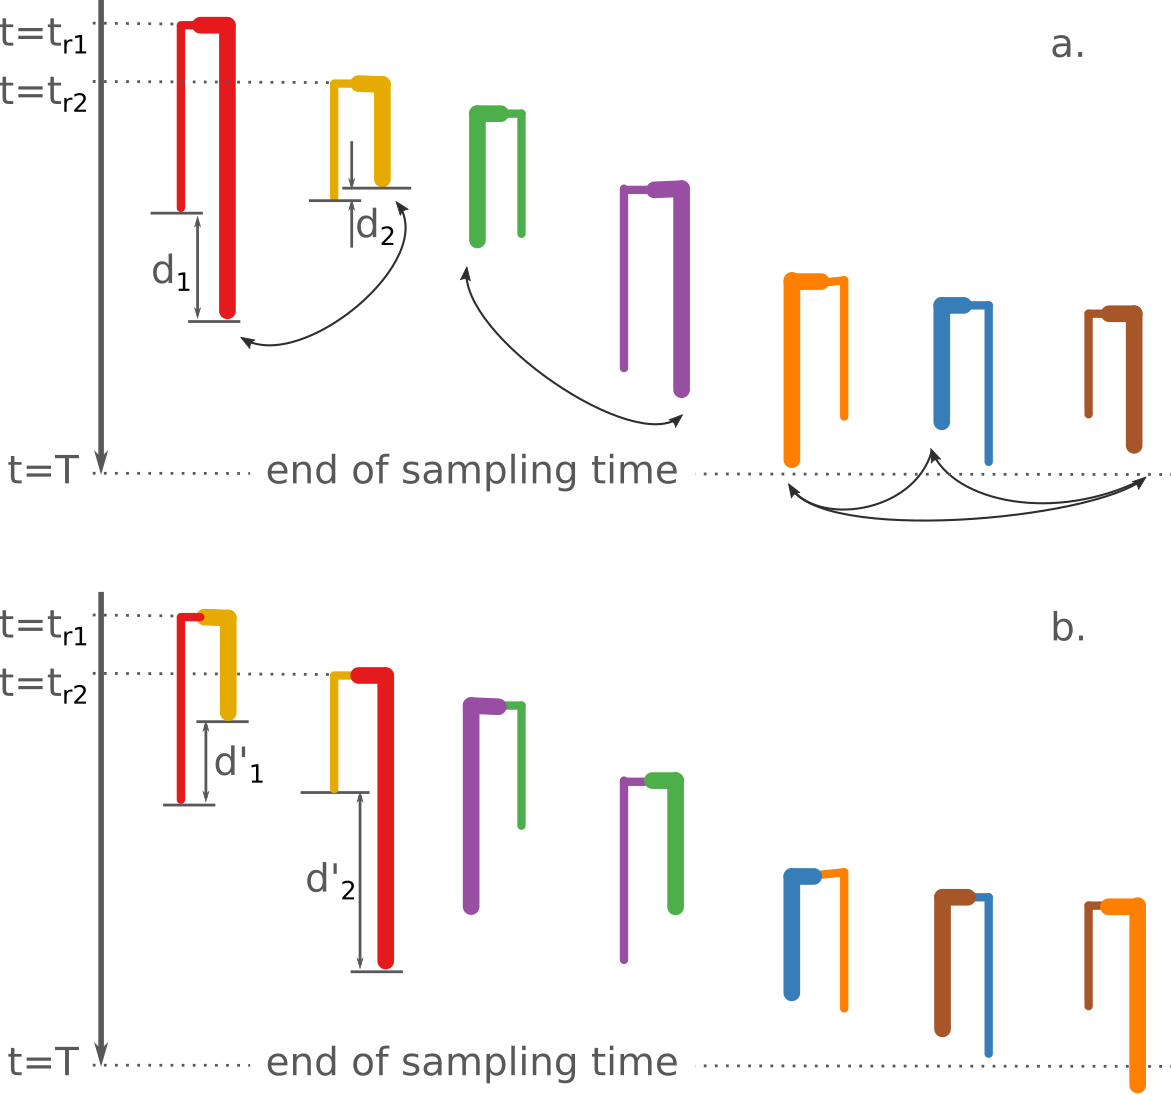
\includegraphics[width=0.8\textwidth]{Fig_cherryswap.png}
\caption{Reshuffled cherry generation. \textbf{a.} Cherries of the original tree sorted by their root times (times of the roots of the two oldest cherries, $t_{r1}$ and $t_{r2}$, are shown on the left). The randomly selected tip is shown with a bold branch for each cherry (e.g. the tip on the right for the leftmost cherry). The tip sampling time differences are shown for the two leftmost cherries ($d_1$ and $d_2$). \textbf{b.} Reshuffled cherries, which were obtained from the original ones by swapping the selected tips between the neighbouring cherry couples (as shown with arrows in a.): the first and the second; the third and the forth. As the total number of cherries (7) is odd, the last three (instead of two) cherries exchanged their selected tips in a cycle. The reshuffled tip sampling time differences are shown for the two leftmost cherries ($d'_1$ and $d'_2$).}
\label{fig:tipswap} 
\end{figure*}

%The reason for which we are constructing a random cherry from the neighbouring instead of any cherries (in terms of root date), is that cherry branch lengths depend on the date of the cherry root. As tip sampling times are bounded from above by the end of the sampling period, the closer the cherry root is to the end of the sampling period, the shorter on average its branches will be (and less time difference they will be able to have in any case). 


\subsection*{Code availability}
We implemented the PN-test in Python 3. It is available as a part of BDPN parameter estimator (see section~\ref{sec:sim}).


\subsection{Performance on simulated data}~\label{sec:test:sim}
To illustrate the PN test performance, we applied it to the trees simulated under three classical MTBD-family models: BD, BDEI (Birth-Death Exposed-Infectious~~\citep{Stadler2014}) and BDSS (Birth-Death with SuperSpreading~\citep{Stadler2013a}), and under their -PN versions: BD-PN, BDEI-PN and BDSS-PN models. (See Fig.~1 in \citet{Voznica2021} for a graphical representation of BD, BDEI and DBSS models and their parameters).

For each model, we generated 100 trees with 500--1\,000 tips with our MTBD/MTBD-PN tree simulator. For each tree the parameter values were drawn randomly within the following bounds:
\begin{itemize}
\item $R_e = \frac{{\lambda}}{{\psi}} \in ]1, 5]$, 
\item removal rate $\psi \in ]1 / 20, 1 / 5]$,
\item sampling probability $\rho \in ]0.1, 0.9]$,
\item \textit{(for -PN models only)} ratio between the partner removal rate after notification and the removal rate $\frac{\phi}{\psi} \in ]50, 500]$,
\item \textit{(for -PN models only)} partner notification probability $\upsilon \in ]0.01/\rho, 0.9]$ (the lower bound was picked this way to ensure that the probability to be a notified partner is at least 0.01 $=\rho \upsilon$),
\item \textit{(for BDEI models only)} becoming-infectious rate (at which an exposed individual becomes infectious) $\mu \in ]0.2, 10]$,
\item \textit{(for BDSS models only)} fraction of superspreaders $f_{SS} = \frac{\lambda_{SS}}{\lambda_{SS} + \lambda_{SN}} \in ]0.05, 0.2]$,
\item \textit{(for BDSS models only)} superspreading transmission ratio $x_{SS} = \frac{\lambda_{SS}}{\lambda_{NS}} = \frac{\lambda_{SN}}{\lambda_{NN}} \in ]3, 10]$.
\end{itemize} 

The common parameters were consistent between models, in a sense that the $i$-th tree under the BDSS model had the same $R_e$, $\psi$ and $\rho$ values as the $i$-th trees under BDSS-PN, BD(-PN) and BDEI(-PN) models; the $i$-th tree under the BDSS-PN model had the same $\phi$ and $\upsilon$ values as the $i$-th trees under BD-PN and BDEI-PN models.

We then run the PN tests on each tree of these 6 datasets. For 98/97/95 out of 100 trees in the BD/BDEI/BDSS dataset the PN test p-value was above $0.05$ (i.e. 98\%/97\%/95\% true negative and 2\%/3\%/5\% false positive results). For 95/95/96 out of 100 trees in the BD-PN/BDEI-PN/BDSS-PN dataset the PN test p-value was below $0.05$ (i.e. 95\%/95\%/96\% true positive and 5\%/5\%/4\% false negative results). These results are summarised in Table~\ref{tbl:pntest}. Our test therefore showed both high specificity and sensitivity.

\begin{table}[!h]\centering
\small
\caption{PN test performance on trees generated under BD, BDEI, BDSS, BD-PN, BDEI-PN and BDSS-PN models (100 trees per model). We report the number of trees for which the PN-test p-value was $<0.05$, $\geq 0.05$, and the mean p-value for each model dataset.}
\begin{tabular}{l|r|r|c}
 & \textbf{p-value $<0.05$} & \textbf{p-value $\geq0.05$} & \textbf{mean p-value} \\
  \midrule
\textbf{BD}& 2 & 98 & 0.479 \\
\textbf{BD-PN}& 95 & 5 & 0.015 \\
  \midrule
\textbf{BDEI}& 3 & 97 & 0.531 \\
\textbf{BDEI-PN}& 95 & 5 & 0.008 \\
  \midrule
\textbf{BDSS}& 5 & 95 & 0.505 \\
\textbf{BDSS-PN}& 96 & 4 & 0.008 \\
\end{tabular}
\label{tbl:pntest}
\end{table}
 

\section{Mathematical formulation of BD and BD-PN models}\label{math}

The BD model can be described with master equations representing the likelihood densities of evolving as on the observed transmission tree, with time $t$ going forward from the root ($t=0$) till the time of the last sampled tip ($t=T$). These likelihood densities depend on the probability $U(t)$ of an unobserved transmission tree that started from one individual at time $t$ and evolved till $T$, without this individual nor any of their induced cases being sampled: 

\begin{equation}
\scriptsize
\begin{cases}
\dot{U}(t) = &\Big(\lambda + \psi\Big) U(t)\; \textit{\color{gray} $\leftarrow$ no event in the next infinitesimal time $\Delta t$ }\\
    &- \lambda U^2(t) \;  \textit{\color{gray} $\leftarrow$ transmission, followed by unsampled evolutions of both subtrees}\\
    &- \psi (1 - \rho)\;  \textit{\color{gray} $\leftarrow$ removal without sampling}\\
U(T) = & 1\;  \textit{\color{gray} $\leftarrow$ the probability to stay unsampled over time 0 is 1} \label{eq:Us}
\end{cases}
\end{equation}


With the equation~(\ref{eq:Us}), we can write down the equation for the probability density $p^{(i)}(t)$ of evolving as on an observed tree branch that finishes at time $t_i$, starting on this branch at a time $t \leq t_i$. The master equations for the BD models were initially developed by ~\citet{Stadler2009}, however what we present here is their branch-specific formulation that we proposed in~\citep{zhukovaFastAccurateMaximumLikelihood2022}:
In our formulation, ${p}^{(i)}(t)$ describes an evolution along a tree branch $i$, without taking into account the branch's subtree. % and provided that we do not know whether the individual at the end of the branch (at time $t_i$) is the same as at time $t$. These two individuals could be different if a hidden transmission, where the donor subtree stayed unobserved, occurred between times $t$ and $t_i$. 

\begin{equation}
\scriptsize
\begin{cases}
\dot{p}^{(i)}(t) = & \Big(\lambda + \psi\Big) p^{(i)}(t)\; \textit{\color{gray} $\leftarrow$ no event in the next infinitesimal time $\Delta t$ }\\
    & - 2 \lambda p^{(i)}(t)U(t)\;  \textit{\color{gray} $\leftarrow$ transmission, where one of the subtrees stayed unsampled}\\
p^{(i)}(t_i) =  &1\;  \textit{\color{gray} $\leftarrow$ the probability of no change over zero time is 1}
\end{cases}\label{eq:p}
\end{equation}


Using this equation, we can calculate the likelihood density $L(\mathscr{T}|\Theta)$ of a tree $\mathscr{T}$ under parameter values $\Theta = \{\lambda, \psi, \rho\}$ as:

\begin{equation}
\scriptsize
\begin{split}
log L(\mathscr{T}|\Theta) =  &\sum\limits_{i \in tips}  log(\psi \rho)  \textit{\color{gray} $\leftarrow$ sampling of tips} \\
 &+\sum\limits_{i \in \stackanchor{\tiny\textit{internal}}{\tiny\textit{nodes}}} log \big(2 \lambda p^{(i0)}(t_i)p^{(i1)}(t_i)\big)   \textit{\color{gray} $\leftarrow$ transmission events, followed by child }\\
 & ~~~~~~~~~~~~~~~~~~~~~~~~~~~~~~~~~~~~~~~~~~~~~~~~~~\textit{\color{gray} branch evolutions (each can be a donor)}  \label{eq:mtbd_tree_likelihood}
\end{split}
\end{equation}



Importantly, the BD model is asymptotically unidentifiable (see Remark 3.4 in~\citep{Stadler2009}). To become identifiable it requires one of its parameters to be fixed. In practice, it is often the sampling probability $\rho$, as it may be approximated from epidemiological data (e.g., the proportion of sampled cases among the declared ones) or the infectious time $\frac{1}{\psi}$ (estimated from observations of infected cases). 



In the classical BD model with incomplete sampling, a branch of the tree corresponds to a virus evolution between the transmission corresponding to the node at the beginning of this branch and either a sampling event (if the branch is external) or a transmission corresponding to the node at the end of the branch (if it is internal). Note, that since sampling is incomplete, hidden transmissions (leading to fully unsampled subtrees) could occur along this branch, where the unsampled subtree could correspond to either donor or recipient.  Hence, we do not know whether the individual at the end of the branch (at time $t_i$) is the same as at any time $t < t_i$ along the branch. These two individuals could be different if a hidden transmission, where the donor subtree stayed unobserved, occurred between times $t$ and $t_i$. $p^{(i)}(t)$ in equations~(\ref{eq:p}) describes an evolution along such a tree branch (with potentially different individuals at times $t$ and (the branch end) $t_i$).

In trees generated by the BD-PN model, however, two other types of branches are possible. Let us consider a tip corresponding to a person A who got sampled at time $t_A$ and successfully notified their partner B (see Fig.~\ref{fig:pn-branches}). According to our model assumption 2, notified individuals are always observed. Hence B must be sampled too (at time $t_B \geq t_A$) and corresponds to a tree tip, while the common ancestor of A and B (AB) corresponds to the transmission between A and B. Therefore the individual on the path between AB and B cannot change (is always B) and only hidden transmissions (from B to someone else) where the recipient subtree stayed unobserved are possible along the branch(es) leading from AB to B (before $t_A$). Note, that non-hidden transmissions are also possible before the notification time $t_A$, and in such a case we know which subtree corresponds to the donor (the one that contains B). Between $t_A$ and $t_B$ no transmission is possible on the branch of B as, according to assumption 3, after notification notified individuals do not transmit further.

We will use an \textbf{oriented (partner) branch probability} $p_o^{(i)}(t)$ for cases when the individual at the end of the branch (or considered time interval) is the same as at time $t$ but might have transmitted to someone else (unobserved) along the way:

\begin{equation}
\scriptsize
\begin{cases}
\dot{p}_o^{(i)}(t) &=~~  \Big(\lambda + \psi\Big) p_o^{(i)}(t)\; \textit{\color{gray} $\leftarrow$ no event in the next infinitesimal time $\Delta t$ }\\
    &~~~ - \lambda p_o^{(i)}(t)U(t)\;  \textit{\color{gray} $\leftarrow$ transmission, where the recipient subtree stayed unsampled}\\
p_o^{(i)}(t_i) &=  1\label{eq:p-o}
\end{cases}
\end{equation}

We will use a \textbf{notified partner branch probability} $p_p^{(i)}(t)$ for cases when the individual at the end of the branch is the partner who got notified at time $t_n < t$:

\begin{equation}
\scriptsize
\begin{cases}
\dot{p}_p^{(i)}(t) &=  \phi p_p^{(i)}(t)\; \textit{\color{gray} $\leftarrow$ no sampling in the next infinitesimal time $\Delta t$ }\\
p_p^{(i)}(t_i) &=  1\label{eq:p-np}
\end{cases}
\end{equation}

Moreover, according to our model assumption 4, only the most recent partner can get notified. Hence, AB must be the parent node of A, and no hidden transmission is possible along the branch AB-A (as otherwise there would have been a partner of A who is more recent than B).

We will use a \textbf{notifier branch probability} $p_n^{(i)}(t)$ for such cases (when no hidden transmission occurred along the branch):

\begin{equation}
\scriptsize
\begin{cases}
\dot{p}_n^{(i)}(t) &=  \Big(\lambda + \psi\Big) p_n^{(i)}(t)\; \textit{\color{gray} $\leftarrow$ no event in the next infinitesimal time $\Delta t$ }\\
p_n^{(i)}(t_i) &= 1\label{eq:p-nh}
\end{cases}
\end{equation}

Note that A could have also ``unsuccessfully'' notified B, if by the time $t_A$, when A decided to notify B, B had already got sampled via the standard procedure or got notified by someone else. In this case nothing changes for the AB-A branch, and the AB-B branch(es) stay oriented. 


\begin{figure*}[tbhp]
\centering 
%\includegraphics[width=0.8\textwidth]{Transmission_tree.png}
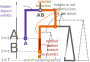
\includegraphics[width=0.6\textwidth]{Fig_PNbranches}
\caption{An example of partner notification in a transmission tree: an individual A got sampled at time $t_A$ (violet tip) and notified their most recent partner B (orange tip). The internal node AB corresponds to the transmission between A and B. The fact that A is the notifier of B implies that there is no hidden event along its branch AB-A, and that in any transmission on the path AB-B the donor is B. Moreover, between the moment of notification ($t_A$) and the moment of sampling  of B ($t_B$) there are no hidden events on the branch B.}
\label{fig:pn-branches} 
\end{figure*}


The equations~\ref{eq:Us}, \ref{eq:p}, \ref{eq:p-o}-\ref{eq:p-nh} have the following closed form solutions:
\begin{equation}
\scriptsize
\begin{split}
&\begin{cases}
U(t) = \frac{\lambda + \psi}{2\lambda} +  \frac{c_1}{2\lambda}\Big(\frac{E_1 - 1}{E_1 + 1}\Big)\\
\\
p^{(i)}(t) = \Big(\frac{E_2 + 1}{E_1 + 1}\Big)^2E_3 \\
\\
p_o^{(i)}(t) =  \frac{E_2 + 1}{E_1 + 1}\sqrt{E_3E_4} \\
\\
p_n^{(i)}(t) =  E_4
\\
p_p^{(i)}(t) =  e^{\phi (t -t_i)}
\end{cases},\\
& \textit{where } c_1 = \sqrt{(\lambda - \psi)^2 + 4 \lambda\psi\rho},\; c_2 = \frac{c_1 + \lambda - \psi}{c_1 - \lambda + \psi},\\
& ~~~~~~~~E_1 = c_2 e^{c_1 (t -T)},\; E_2 = c_2 e^{c_1 (t_i -T)},\; E_3 = e^{c_1 (t -t_i)}, \; E_4 =  e^{(\lambda + \psi) (t -t_i)}\\
\end{split}\label{eq:ps}
\end{equation}



\subsection{BD-PN tree likelihood density} 

Using the formulas~(\ref{eq:ps}), we can calculate the likelihood density of a tree using a pruning algorithm~\citep{10.1093/sysbio/22.3.240}. For each visited node $i$ we calculate the likelihood density of its subtree for two cases depending on their receiving-a-notification status (shown with the first superscript, $^{\not{n}}$ or $^n$). In the first case,  $l^{(\not{n})}(i)$, the branch $ji$ connecting $i$ it to its parent node $j$ corresponds to an unnotified individual. In the second case, $l^{(n)}(i, r)$, the branch $ji$ corresponds to an (eventually) notified partner (notified by the individual corresponding to a tip $r$ at time $t_r$). If $i$ is a tip, we additionally consider whether the corresponding individual notified their most recent partner or not (shown with the second superscript, $^n$ or $^{\not{n}}$). For instance, $l^{(\not{n},n)}(i)$ represents the case where the tip $i$ was not notified but notified their partner. Note that if the tip $i$ was notified by their partner $r$, we need to consider two possibilities: (1) when $t_r \leq t_i$, and hence the notification was successful at provoking $i$'s diagnostics and sampling; and (2) when $t_r > t_i$, and hence by the time of notification by $r$ $i$ already got sampled by other means.

The tree $\mathscr{T}$ likelihood density $\mathscr{L}(\mathscr{T}|\Theta)$ under BD-PN model with parameters $\Theta=\{\lambda, \psi, \rho, \phi, \upsilon\}$ can be calculated as $l^{(\not{n})}(root)$, as the root can only correspond to an unnotified individual (since there was no observed transmission before it).

We will now describe the subtree likelihood density calculation case by case.

\subsubsection*{Case 1: $i$ is a tip} 

For a tip $i$ with a parent node $j$ the subtree likelihood density values can be calculated as:
\begin{equation}
\scriptsize
\begin{array}{ll}
l^{(\not{n},\not{n})}(i) &= p^{(i)}(t_j)\psi\rho (1-\upsilon) \textit{\color{gray} ~i.e. $i$ was not notified and did not notify}\\
& \textit{\color{gray} (standard branch evolution followed by sampling and no notification)}\\
\\
l^{(\not{n},n)}(i) &= p_n^{(i)}(t_j)\psi\rho
\upsilon \textit{\color{gray} ~i.e. $i$ was not notified but notified their most recent patner}\\
& \textit{\color{gray} (notifier branch evolution followed by sampling and notification)}\\
\\
l^{(n,\not{n})}(i,r) &= \begin{cases}
0 \textit{\color{gray} ~if $t_r < t_j$}\\
\textit{\color{gray} (not possible as once notified partners do not transmit)}\\
\\
p_o^{(i)}(t_j)\psi\rho(1 - \upsilon) \textit{\color{gray} ~if $i$ got notified at time $t_r > t_i$ and did not notify}\\
\textit{\color{gray} (oriented (partner) branch evolution followed by standard sampling and no notification)}\\
\\
p_o^{(r)}(t_j) p_p^{(i)}(t_r) \phi (1-\upsilon) \textit{\color{gray} ~if $i$ got notified at time $t_j \leq t_r \leq t_i$ and did not notify}\\
\textit{\color{gray} (oriented (partner) branch evolution followed by} \\
\textit{\color{gray}~notified partner branch evolution,} \\
\textit{\color{gray}~notification-provoked sampling and no notification)}\\
\end{cases}\\
\\
l^{(n,n)}(i,r) &= \begin{cases}0 \textit{\color{gray} ~if $t_r < t_j$}\\
\textit{\color{gray} (not possible as once notified partners do not transmit)}\\
\\
p_n^{(i)}(t_j)\psi\rho\upsilon \textit{\color{gray} ~if $i$ got notified at time $t_r > t_i$ and notified their most recent patner}\\
\textit{\color{gray} (notifier branch evolution followed by standard sampling and  notification)}\\
\\
p_n^{(r)}(t_j) p_p^{(i)}(t_r) \phi \upsilon \textit{\color{gray} ~if $i$ got notified at time $t_j \leq t_r \leq t_i$ and notified}\\
\textit{\color{gray} (notifier branch evolution followed by} \\
\textit{\color{gray}~notified partner branch evolution,} \\
\textit{\color{gray}~notification-provoked sampling and notification)}\\
\end{cases}\\
\end{array}
\label{eq:tip}
\end{equation}

\subsubsection*{Case 2: $i$ is an internal node} 
Let us now consider an internal node $i$ with two child nodes, $i_0$ and $i_1$. 

\subsubsection*{Case 2.1: $i$ is an unnotified internal node} 
We will start with the configuration where the $i$'s branch corresponds to an unnotified individual. Hence the $i$'s branch evolution is represented by $p^{(i)}(t_j)$ with a transmission event at the end of it, where each of the child branches can correspond to the donor (probability density of $2\lambda$). We will consider three possibilities: (1) when both $i_0$ and $i_1$ are internal nodes; (2) when both $i_0$ and $i_1$ are tips; and (3) when one of them is an internal node and the other one is a tip.

%Note that a notification will only be possible if the notifying branch is external as the notifier only notifies the most recent partner, i.e. the transmission corresponds to the notifier's parent node.

\subsubsection*{Case 2.1.1: $i$ is an unnotified internal node with internal-node children $i0$ and $i1$}

First, let's assume that $i_0$ and $i_1$ are internal. Then none of them can be a notifier (since notifiers correspond to tips), and hence none of them is notified (as $i$ is also unnotified):

\begin{equation}
\scriptsize
l^{(\not{n})}(i) = p^{(i)}(t_j) 2\lambda l^{(\not{n})}(i_0)l^{(\not{n})}(i_1) \label{eq:lu-int-int}
\end{equation}

\subsubsection*{Case 2.1.2: $i$ is an unnotified internal node with tip children $i0$ and $i1$}

Secondly, let's assume that $i_0$ and $i_1$ are tips. Then each of them could have notified the other one:

\begin{equation}
\scriptsize
\begin{split}
l^{(\not{n})}(i) = p^{i}(t_j) 2\lambda \cdot 
\Big(&~~~~l^{(\not{n},\not{n})}(i_0)l^{(\not{n},\not{n})}(i_1) \textit{\color{gray}~$\leftarrow$ neigher $i_0$ nor $i_1$ notified} \\
&+ l^{(\not{n},n)}(i_0)l^{(n,\not{n})}(i_1,i_0) \textit{\color{gray}~$\leftarrow$ $i_0$ notified $i_1$ and $i_1$ did not notify} \\
&+ l^{(n,\not{n})}(i_0,i_1)l^{(\not{n},n)}(i_1) \textit{\color{gray}~$\leftarrow$ $i_0$ did not notify, but $i_1$ notified $i_0$} \\
&+ l^{(n,n)}(i_0,i1)l^{(n,n)}(i_1,i_0)~~\Big) \textit{\color{gray}~$\leftarrow$ $i_1$ and $i_0$ notified each other} \\
\end{split}\label{eq:lu-tip-tip}
\end{equation}

\subsubsection*{Case 2.1.3: $i$ is an unnotified internal node whose children are a tip and an internal node}
Lastly, let's assume that $i_0$ is a tip and $i_1$ is internal (the scenario where $i_1$ is a tip and $i_0$ is internal can be obtained by swapping the labels). Then $i_0$ could have notified $i_1$:


\begin{equation}
\scriptsize
\begin{split}
l^{(\not{n})}(i) = p^{i}(t_j) 2\lambda \cdot 
\Big(&~~~l^{(\not{n},\not{n})}(i_0)l^{(\not{n})}(i_1) \textit{\color{gray}~$\leftarrow$ $i_0$ did not notify $i_1$ } \\
&+ l^{(\not{n},n)}(i_0)l^{(n)}(i_1,i_0)~~\Big) \textit{\color{gray}~$\leftarrow$ $i_0$ notified $i_1$} \\
\end{split}\label{eq:lu-int-tip}
\end{equation}

\subsubsection*{Case 2.2: $i$ is an (eventually notified) partner internal node} 

In the other case an internal node $i$ corresponds to a partner who will eventually get notified by a tip $r$. In this case the individual on the path connecting $i$ to its common ancestor $ir$ with the notifier tip $r$ (corresponding to the transmission between $r$ and $i$) stays the same (the partner). Hence, all the transmissions on this path are oriented and correspond to the partner transmitting to another recipient individual. In particular, the $i$'s branch evolution is represented by $p_o^{(i)}(t_j)$ with a transmission event at the end of it, where the donor is known (probability density of $\lambda$): The donor corresponds to the subtree containing the tip representing the sampling of the individual $i$. %Moreover, this recipient's branch cannot be notified by our partner (as in our model notified partners do not notify further):
Again, we will consider three possibilities for $i$'s child nodes: (1) when both $i_0$ and $i_1$ are internal nodes; (2) when both $i_0$ and $i_1$ are tips; and (3) when one of them is an internal node and the other one is a tip.

In any of these scenarios, the notification must have happened after the partner tip branch start (as one of the model assumptions is that partners do not transmit after notification). Hence:
\begin{equation}
\scriptsize
l^{(n)}(i, r) = 0 \textit{\color{gray}~if $t_i > t_r$} \\
\label{eq:lp-zero}
\end{equation}

\subsubsection*{Case 2.2.1: $i$ is a partner internal node with internal-node children $i0$ and $i1$} 

First, let's assume that $i_0$ and $i_1$ are internal. Then none of them can be a notifier (since notifiers correspond to tips), and hence exactly one of them is notified (by $r$):

\begin{equation}
\scriptsize
\begin{split}
l^{(n)}(i, r) = p_o^{(i)}(t_j) \lambda \cdot
\Big(&~~~l^{(n)}(i_0,r)l^{(\not{n})}(i_1) \textit{\color{gray}~$\leftarrow$ $i_0$ is notified by $r$} \\
& + l^{(\not{n})}(i_0)l^{(n)}(i_1,r)~~\Big) \textit{\color{gray}~$\leftarrow$ $i_1$ is notified by $r$} \\
 \end{split}
\label{eq:lp-int-int}
\end{equation}

\subsubsection*{Case 2.2.2: $i$ is a partner internal node with tip children $i0$ and $i1$} 
Secondly, let's assume that $i_0$ and $i_1$ are tips. Then each of them could have notified the other one (in addition to one of them being notified by $r$):

 
\begin{equation}
\scriptsize
\begin{split}
l^{(n)}(i, r) = p_o^{(i)}(t_j) \lambda \cdot
\Big(~~~&l^{(n,\not{n})}(i_0,first(r,i_1))l^{(\not{n},n)}(i_1) \textit{\color{gray}~$\leftarrow$ $r$ and $i_1$ notified $i_0$, $i_0$ did not notify} \\
&+ l^{(n,n)}(i_0,first(r,i_1))l^{(n,n)}(i_1, i_0) \textit{\color{gray}~$\leftarrow$ $r$ and $i_1$ notified $i_0$, $i_0$ notified $i_1$} \\
&+l^{(\not{n},n)}(i_0)l^{(n,\not{n})}(i_1,first(r,i_0)) \textit{\color{gray}~$\leftarrow$ $r$ and $i_0$ notified $i_1$, $i_1$ did not notify} \\
&+ l^{(n,n)}(i_0, i_1)l^{(n,n)}(i_1,first(r,i_0)) \textit{\color{gray}~$\leftarrow$ $r$ and $i_0$ notified $i_1$, $i_1$ notified $i_0$} \\
&+l^{(n,n)}(i_0,r)l^{(n,\not{n})}(i_1, i_0) \textit{\color{gray}~$\leftarrow$ $r$ notified $i_0$, $i_0$ notified $i_1$, $i_1$ did not notify} \\
& + l^{(n,\not{n})}(i_0, i_1)l^{(n,n)}(i_1,r) \textit{\color{gray}~$\leftarrow$ $r$ notified $i_1$, $i_1$ notified $i_0$, $i_0$ did not notify} \\
&+l^{(n,\not{n})}(i_0,r)l^{(\not{n},\not{n})}(i_1) \textit{\color{gray}~$\leftarrow$ $r$ notified $i_0$, $i_0$ and $i_1$ did not notify} \\
& + l^{(\not{n},\not{n})}(i_0)l^{(n,\not{n})}(i_1,r)~~\Big) \textit{\color{gray}~$\leftarrow$ $r$ notified $i_1$, $i_0$ and $i_1$ did not notify}, \\
\textit{\color{gray}~where } &\color{gray}first(a,b) = 
\begin{cases}
a \textit{~if $t_a \leq t_b$}\\
b \textit{~if $t_a > t_b$.}
\end{cases} 
 \end{split}
\label{eq:lu-tip-tip}
\end{equation}


\subsubsection*{Case 2.2.3: $i$ is a partner internal node whose children are a tip and an internal node}
Lastly, let's assume that $i_0$ is a tip and $i_1$ is internal (the scenario where $i_1$ is a tip and $i_0$ is internal can be obtained by swapping the labels). Then $i_0$ could have notified $i_1$ (in addition to one of them being notified by $r$):


\begin{equation}
\scriptsize
\begin{split}
l^{(n)}(i, r) = p_o^{(i)}(t_j) \lambda \cdot
\Big(~~~&l^{(n,n)}(i_0,r)l^{(n)}(i_1,i_0) \textit{\color{gray}~$\leftarrow$ $r$ notified $i_0$, $i_0$  notified $i_1$} \\
& + l^{(n,\not{n})}(i_0,r)l^{(\not{n})}(i_1) \textit{\color{gray}~$\leftarrow$  $r$ notified $i_0$, $i_0$ did not notify} \\
& +l^{(\not{n}, n)}(i_0)l^{(n)}(i_1,first(r,i_0)) \textit{\color{gray}~$\leftarrow$ both $r$ and $i_0$ notified $i_1$} \\
& + l^{(\not{n},\not{n})}(i_0)l^{(n)}(i_1,r)~~\Big) \textit{\color{gray}~$\leftarrow$ $r$ notified $i_1$, $i_0$ did not notify}, \\
\textit{\color{gray}~where } &\color{gray}first(a,b) = 
\begin{cases}
a \textit{~if $t_a \leq t_b$}\\
b \textit{~if $t_a > t_b$.}
\end{cases} 
 \end{split}
\label{eq:lp-tip-int}
\end{equation}


Note that $l^{(n)}(i, r)$ depends on the notifier $r$ and can only be calculated once the notification time is known, i.e. once we have climbed to an internal node corresponding to the transmission between the notifier (corresponding to one of its children, must be a tip) and the partner (the other child). The calculation is done recursively by descending into the subtree. However, as all the unotified equation parts, $l^{(\not{n})}(i)$, only depend on the corresponding node $i$, they can be pre-calculated and reused to speed up the recursive steps.



\bigskip



%The computational of $\mathscr{L}(\mathscr{T}|\Theta)$ includes $O(N^2)$ resolutions of system~(\ref{eq:p}) (for different times and initial conditions) in the worst case (caterpillar tree) and $O(NlogN)$ in the best case (for a balanced tree), where $N$ is the number of tips in $\mathscr{T}$.


\subsection{Extension to forests}

As we previously described in~\citep{zhukovaFastAccurateMaximumLikelihood2022}, the likelihood calculation with MTBD models can be easily extended to forests. This extension applies also to the BD-PN model. Forests are useful for cases when a (sub-)epidemic started with several infected individuals (e.g. due to multiple pathogen introductions to a country of interest or due to a change of health policies leading to a change in parameter values).

In this case the (sub-)epidemic leads to a forest $\mathscr{F}$ of $f$ observed trees: $\mathscr{T}_1, \ldots, \mathscr{T}_f$. The forest $\mathscr{F}$ might also include a certain number $u$ of unobserved trees, for which none of their tips got sampled.
Forest likelihood formula hence combines the likelihoods of $f$ observed and $u$ hidden trees, and can be represented in a logarithmic form~(\ref{eq:forest_likelihood}). The tree likelihood formula %[\ref{eq:tree_likelihood}] 
is its special case, where $f=1$ and $u=0$. 

%As our application to Ebola data (see~Application) shows, $u$ is an important parameter: while the results are not very sensible to slight $u$ variations, ignoring it completely (e.g. using $u=0$ instead of $u \approx 500$ in our example) can change the inferences.

\begin{equation}
\begin{split}
logL(\mathscr{F}|\Theta,u)&=u\,logU_{hidden}(\Theta) + \sum\limits_{j=1}^f logL(\mathscr{T}_j|\Theta), \\
\textit{ where }& U_{hidden}(\Theta)=\sum\limits_{s=1}^{d}\pi_s U_s(t_{start}),\\
\textit{ and }& t_{start} \textit{ is the (potentially averaged) start time of the hidden trees.}
\end{split} \label{eq:forest_likelihood} 
\end{equation}

For given model parameter values $\Theta$ we can estimate the number of hidden trees $u$ from the number of observed trees $f$ as:
\begin{equation}
u = f \frac{U_{hidden}(\Theta)}{1 - U_{hidden}(\Theta)}\label{eq:u} 
\end{equation}


\section{BD-PN parameter and CI estimator}\label{sec:sim}
We implemented a parameter estimator for the BD-PN model (which we called bdpn). It estimates the BD-PN model parameters  $\Theta = (\lambda,\psi,\phi,\rho,\upsilon) \in \mathbb{R}^5$ for a forest $\mathscr{F}$ comprising $f \geq 1$ observed trees in the maximum-likelihood framework, where one of the BD parameters ($\lambda,\psi$ or $\rho$) is fixed (for identifiability reasons). 

Once the optimal parameter values are found, we calculate their confidence intervals (CIs) using Wilks' method~\citep{Wilks1938}.
For each non-fixed parameter $p \in \Theta$, we calculate its $95\%$-CI as including the values $\tilde{p}$ such that $log L(\mathscr{F}|\Theta_{opt|p=\tilde{p}}) > log L(\mathscr{F}| \Theta_{opt}) - \chi^2_1(0.95) / 2$, where $\chi^2_1(0.95)$ is the value of chi-squared distribution with 1 degree of freedom corresponding to the significance level of $0.95$ (i.e., $\sim3.84$). $\Theta_{opt|p=\tilde{p}}$ corresponds to the maximum-likelihood value for the other non-fixed parameters when $p = \tilde{p}$. 

\subsection*{Code availability}
The BD-PN parameter estimator is implemented in Python 3. It uses ETE 3 framework for tree manipulation~\citep{Huerta-Cepas2016} and NumPy package for array operations~\citep{harris_array_2020}. 

It is available as a command-line program and a Python 3 package via PyPi (\href{https://pypi.org/project/bdpn}{bdpn}), and via Docker/Singularity (\href{https://hub.docker.com/r/evolbioinfo/bdpn/tags}{evolbioinfo/bdpn}). Its source code and the installation and usage documentation are available on GitHub at \href{https://github.com/evolbioinfo/bdpn}{github.com/evolbioinfo/bdpn}.

\subsection{Performance on simulated data}

To assess the performance of our maximum-likelihood estimator for the BD-PN model, we used the 100 trees with 500--1\,000 tips simulated under the BD-PN model as described in subsection~\ref{sec:test:sim}.

We applied bdpn to each of the trees three times: fixing each of the BD parameters ($\lambda,\psi$ or $\rho$) to its real value (for identifiability). 


As expected with a maximum likelihood estimator, the tree likelihoods for the estimated parameter values were higher than or equal to the tree likelihoods for the real parameter values in all the settings.

We calculated the relative error (normalized distance between the estimated and the target values: $\frac{|estimated - target|}{target}$) and the relative bias ($\frac{estimated - target}{target}$) for each parameter on each tree (Fig.~\ref{fig:sim}). 
Average relative errors were the lowest when $\psi$ or $\rho$ were fixed: $\leq 10\%$  for all the parameters. The worst performance was obtained with $\lambda$ being fixed: in this setting the estimator tends to underestimate $\psi$ and overestimate $\rho$.
%The hardest parameter to estimate in all the settings (relative errors $\approx 15\%$, with a tendency to underestimation). 

As with the point estimates, CI estimates were the best when $\psi$ or $\rho$ were fixed, and the worst when $\lambda$ was fixed (see Table~\ref{tbl:ci}). The relative width of the CIs ($\frac{value_{97.5\%} - value_{2.5\%}}{value}$) varied between 11\% for $\lambda$ estimates and 32\% for $\phi$ estimates (in all the settings).

\begin{figure}[!pht]
\centering 
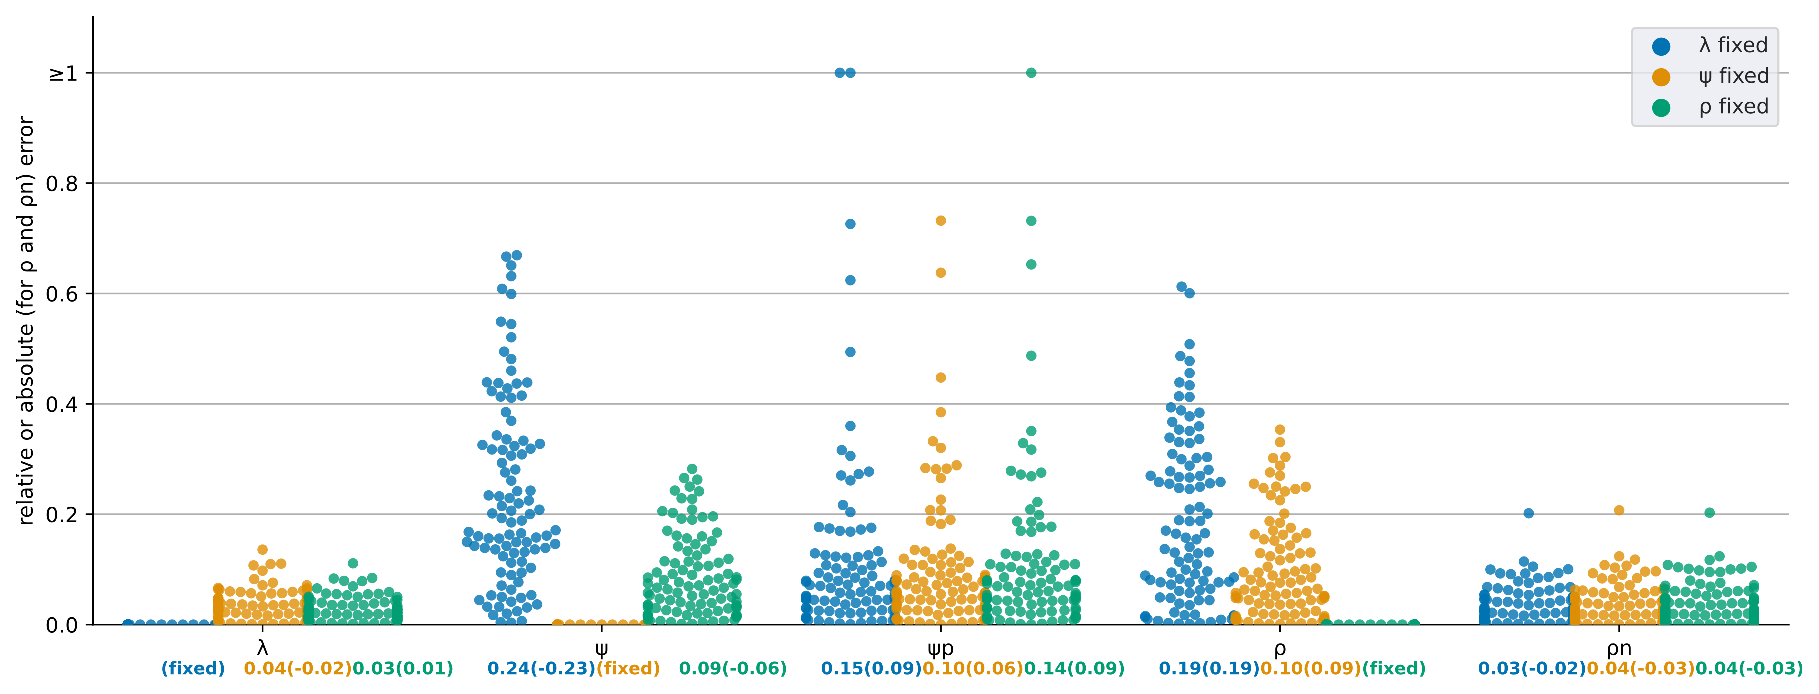
\includegraphics[width=1\textwidth]{Fig_errors.eps}
\caption{Comparison of inference accuracy of bdpn on a data set of 100 trees of 500--1\,000 tips each, with either $\lambda$ (blue), $\psi$ (orange) or $\rho$ (green) parameter being fixed to its real value.
We show the swarmplots (coloured by fixed parameter) of relative errors for each test tree and parameter, which are measured as the normalized distance between the estimate and the real value. Average relative error (and in parentheses average relative bias) are displayed for each parameter and method below their swarmplot. For $\rho$ and $\upsilon$ absolute values are shown instead of normalized ones. } 
\label{fig:sim} 
\end{figure}
 
 \begin{table}[!h]\centering
\small
\caption{Percentage of simulated trees for which the real parameter values were withing the estimated 95\% CIs. \smallskip}
\begin{tabular}{c|ccc}
\textbf{parameter} & \textbf{$\lambda$ fixed} & \textbf{$\psi$ fixed} & \textbf{$\rho$ fixed} \\
\toprule 
 $\lambda$ & -- &  76\% & 96\% \\
 $\psi$ & 22\% & -- & 78\% \\
 $\rho$ & 16\% & 55\%  & -- \\
 $\phi$ & 70\% & 93\% & 94\% \\
 $\upsilon$ & 21\% & 68\% & 63\% \\
\bottomrule
\end{tabular}
\label{tbl:ci}
\end{table}


\subsection{Application: HIV-B epidemic in the UK}
We applied our estimator to asses the partner notification in HIV-infected patients in the UK. We used the phylogenetic tree from our recent study of HIV drug resistance in the UK~\citep{zhukovaModelingDrugResistance2023}. The tree tips represent viruses sampled from 40\,055 individuals between 1996 and 2016. The samples used for the tree reconstruction were obtained from the UK HIV Drug resistance database~\citep{Dunn2007}. The sampling date metadata for these samples were month-specific (e.g. Aug 2015), hence potentially creating simultaneous sampling dates for cases, which were sampled on different days of the month. To avoid this issue we randomly selected a date within the specified month for each sample, and time-scaled the tree with LSD2~\citep{To2016} (v2.4.1, strict molecular clock with outlier removal). We repeated this time-scaling procedure 10 times, obtaining 10 trees with slightly different branch lengths and root dates between Oct 5 and Nov 11, 1962.

Between 2012 and 2015, in the UK antiretroviral treatment (ART) of HIV-infected individuals  was initiated when their CD4 count dropped below 350 cells/mL~\citep{williamsBritishHIVAssociation2012}. However ``if a patient with a CD4 cell count > 350 cells/mL wishes to start ART to reduce the risk of transmission to partners, this decision is respected and ART is started''~\citep{williamsBritishHIVAssociation2012}. Before 2012, treatment started with an even lower CD4 (i.e. later). The British HIV Association 2015 guidelines recommend all individuals with suspected or diagnosed primary HIV infection ``are offered immediate ART''~\citep{churchillBritishHIVAssociation2016}. To have a more homogeneous setting in terms of access to ART, awareness of the HIV infection, etc., we cut the dated trees between 2012 and 2015. We then applied the PN-test and estimated the BD-PN parameters on these 2012--2015 forests. 

The PN-test values were below 0.05 for all the forests (value between $0.01$ and $0.04$), suggesting the presence of partner notification.

To estimate the BD-PN parameter values, we needed to fix one of the parameters for model identifiability. We therefore estimated the base sampling probability $\rho$ as follows. According to the \href{https://webarchive.nationalarchives.gov.uk/ukgwa/20181112132123mp_/https://assets.publishing.service.gov.uk/government/uploads/system/uploads/attachment_data/file/602942/HIV_in_the_UK_report.pdf}{``Towards elimination of HIV transmission, AIDS and HIV-related deaths in the UK''}
 report, the estimated total number of people living with HIV in the UK in 2015 was 101\,200 (97\,500 to 105\,700). % in 2012 this number was 98\,400 (93\,500-104\,300) [\href{HIV in the United Kingdom: 2013 Report}{https://webarchive.nationalarchives.gov.uk/ukgwa/20181112133715mp_/https://assets.publishing.service.gov.uk/government/uploads/system/uploads/attachment_data/file/326601/HIV_annual_report_2013.pdf}]. Moreover these document report about 400 HIV-related deaths per year. 
According to our estimate~\citep{zhukovaModelingDrugResistance2023}, 66.5\% of the HIV-infected individuals in the UK were infected with HIV-B. We hence estimated that in 2015 67\,298 (64\,837, 70\,291) people were living with HIV-B. Our trees contained 39\,047 tips sampled by the end of 2015, and therefore account for about 58\% (56\%, 60\%) of the total number of individuals living with HIV-B in the UK. We hence fixed the sampling probability $\rho$ to 0.58. %However this estimate does not take into account deaths of the HIV-infected individuals over the years, which would increase the total number of HIV-infected individuals by 2015, and decrease the proportion of individuals represented by our tree. We therefore tested several sampling probabilities $\rho=$0.6; 0.5; 0.4.
 
 
Using $\rho=0.58$, we estimated the following parameter values: $\lambda=0.53$, $\psi=0.43$, $\phi=23-59$, $\upsilon=0.006-0.007$, which corresponds to $R_e = 1.2$, infectious time $\frac{1}{\psi} = 2.3$ years, and about 6--16 days between partner notification and their sampling. The results are consistent between 10 forests and shown in Table~\ref{tbl:uk}. %The results for $\rho=0.4$ and for $\rho=0.6$ were similar: $R_e$ of respectively $1.5$ and 
%$1.3$, infectious time of $5.1$ and $5.6$ years, partner notification probability of $0.033$ in both cases and about 2 days between partner notification and their sampling.
 
The average time of HIV progression to AIDs in the absence of treatment is 10 years, which could serve as an estimate of the infectious time. However, in the UK, 95\% of infected population is on antiretroviral treatment, which, when taken properly, prevents transmission. Hence, the average infectious time represents the average time before starting treatment. Our estimate is approximately 2.3 years. 

\begin{table}
\caption{BD-PN model parameters estimated for UK HIV-1 B epidemic between 2012 and 2015, assuming that our data represents 58\% of infected cases ($\rho=0.58$).}
\label{tbl:uk}
\begin{tabular}{c|cc|cccc}
&&&&infectious&partner&\\
fo-&num.&num.&&time&removal t.&\\
rest&tips&trees&$R_e$&$\frac{1}{\psi}$ [years]& $\frac{1}{\phi}$ [days]&$\upsilon$\\
\toprule
 $1$ & $11\,117$ & $8\,838$& $1.24\;[1.22-1.27]$& $2.34\;[2.29-2.39]$& $8\;[5-12]$& $0.007\;[0.004-0.010]$ \\
 $2$ & $11\,109$ & $8\,833$& $1.24\;[1.21-1.27]$& $2.33\;[2.28-2.39]$& $6\;[4-10]$& $0.006\;[0.003-0.009]$ \\
 $3$ & $11\,122$ & $8\,844$& $1.24\;[1.22-1.27]$& $2.34\;[2.28-2.39]$& $16\;[3-18]$& $0.006\;[0.003-0.010]$ \\
 $4$ & $11\,119$ & $8\,838$& $1.24\;[1.22-1.27]$& $2.34\;[2.28-2.39]$& $7\;[5-11]$& $0.007\;[0.004-0.010]$ \\
 $5$ & $11\,116$ & $8\,829$& $1.24\;[1.22-1.27]$& $2.33\;[2.28-2.39]$& $9\;[6-13]$& $0.006\;[0.003-0.009]$ \\
 $6$ & $11\,111$ & $8\,827$& $1.24\;[1.22-1.27]$& $2.34\;[2.28-2.39]$& $8\;[5-12]$& $0.006\;[0.003-0.009]$ \\
 $7$ & $11\,119$ & $8\,838$& $1.24\;[1.22-1.27]$& $2.33\;[2.28-2.39]$& $7\;[5-11]$& $0.006\;[0.003-0.009]$ \\
 $8$ & $11111$ & $8\,830$& $1.24\;[1.21-1.27]$& $2.33\;[2.28-2.39]$& $6\;[4-11]$& $0.006\;[0.003-0.008]$ \\
 $9$ & $11\,120$ & $8\,833$& $1.24\;[1.21-1.27]$& $2.33\;[2.28-2.39]$& $7\;[4-12]$& $0.006\;[0.003-0.009]$ \\
 $10$ & $11\,112$ & $8\,827$& $1.25\;[1.22-1.27]$& $2.34\;[2.29-2.39]$& $7\;[5-11]$& $0.006\;[0.004-0.009]$ \\
 \bottomrule
 \end{tabular}
 \end{table}



\section{Discussion}
\label{disc}

We proposed an extension of the phylodynamic birth-death model that accounts for non-random sampling due to partner notification (BD-PN). In real-life epidemics, detected infected individuals might notify the people whom they think they might have infected or got infected by, and who in turn might get tested and detected in a much faster and non-random way. Our model accounts for this scenario.

The -PN extension adds two constant parameters to the classical BD model: the probability of partner notification $p_n$ and the partner detection rate $\phi$. It can also be applied to a more general, multi-type birth-death (MTBD) model framework, which accounts for heterogeneity in the infected population (see Appendix). 

We developed a mathematical framework for calculation of the likelihood density of a transmission tree (approximated by a time-scaled phylogenetic tree) under the BD-PN model, and implemented a maximum-likelihood BD-PN parameter estimator based on this framework. The advantage of the BD-PN model is that the differential equations describing it have closed-form solutions, which are quick to calculate and do not require numerical approximation (as is the case for more complex MTBD models). Tests on simulated data show that our estimator robustly infers model parameter values and their CIs in the setting when the duration of the infectious period $\frac{1}{\psi}$ or the base sampling probability $\rho$ if fixed. Fixing one of the model parameters is needed for identifiability. In practice, $\rho$ and $\frac{1}{\psi}$ may often be approximated from epidemiological data, e.g., as the proportion of sampled cases among the declared ones (for $\rho$), or estimated from observations of infected cases ($\frac{1}{\psi}$). 

We also developed a PN-test allowing to distinguish between trees generated under models with and without partner notification. Its application to simulated data showed high sensitivity and specificity. 

We applied the PN-test our estimator to the HIV-1 B epidemic in the UK, between 2012 and 2015. The test detected the presence of partner notification. The obtained estimates of epidemiological parameters are in agreement with what we now know about this epidemic (e.g., $R_e \approx 1.2$ ). We estimated a modest partner notification probability $\upsilon \in [0.003-0.1]$, and rapid notified partner detection ($3-18$ days vs $\approx2.3$ years for detection under the standard random procedure).

The BD-PN model is the first step towards accounting for non-random sampling in phylodynamic models. In order to reduce its mathematical complexity (having closed-form solutions for its differential equations) and make parameter estimation fast, we made several assumptions: (i) that only detected individuals can notify their partner; (ii) only the most recent partner can get notified; (iii) after the notification, notified partners do not transmit further; and (iv) notified partners are always sampled upon removal (i.e., observed in the transmission tree). These assumptions may be too simple to fully grasp the real partner notification process and should be relaxed in the future work. Another needed extension should account for population heterogeneity (i.e., MTBD-PN). As it is much easier to implement a tree simulator with a complex model than to derive its likelihood, a promising path to take for future -PN model developments would be using deep learning (e.g., adding new models to PhyloDeep~\citep{Voznica2021}). 



\bibliographystyle{plainnat}
\bibliography{refs}

\section{Appendix}


\subsection{MTBD-PN tree simulator}

Our tree simulator generates sampled transmission trees under MTBD and MTBD-PN models (with $m$ states). It is Gillespie-based, generates state change, transmission and removal times, and only reconstructs the sampled parts of the tree to save memory and increase speed.  

The simulator iterates through occurring events till either time or sampled tip number limit is reached. 
It keeps updating an array $C = [c_1, \ldots, c_m]$ of counts of currently infected individuals (i.e. non-removed) in different states; an array $S = [s_1, \ldots, s_m]$ of counts of sampled individuals in different states; as well as a mapping $M$ between states and ids of currently infected individuals in those states, and a mapping $N$ between states and ids of sampled individuals in those states.  In the beginning ($t=0$) the only infected individual corresponds to the root: $c_k = 0 \;\forall k \neq state(root), \;c_{state(root)} = 1; \;M_k = \emptyset \; \forall k \neq state(root)$, $ \; M_{state(root)} = \{root\}$, and no individual is sampled: $s_k=0,\;N_k = \emptyset \; \forall 1 \leq k \leq m$.

At each iteration the algorithm (1) calculates the time of the next event; (2) chooses the type of this event and the the individual involved in it; (3) updates the counts and the mappings according to the event and records its time.

At step 1, to calculate the time of the next event, we (i) calculate the total rate $r$ as a sum of total state change, transmission and transition rates: $r = r^{(\mu)} + r^{(\lambda)} + r^{(\psi)}$, where $r^{(\mu)} = \sum\limits_{k=1}^{m} c_k \sum\limits_{r=1}^{m} \mu_{kr}$, $r^{(\lambda)} = \sum\limits_{k=1}^{m} c_k \sum\limits_{r=1}^{m} \lambda_{kr}$, and $r^{(\psi)} = \sum\limits_{k=1}^{m} c_k \psi_{k}$; (ii) draw $\Delta t$ from the exponential distribution with rate $r$; (iii) update the current time to $t + \Delta t$.

At step 2, to chose the type of the event, we draw a value $v$ (uniformly) from an interval $[0, r[$. This interval can be seen as composed of subintervals corresponding to each possible event, where the width of each subinterval is defined by the corresponding rate and infected individual count, e.g. the subinterval corresponding to a transmission from $k$ to $r$ has a width of $\lambda_{kr}c_k$. The subinterval in which $v$ is located defines the event type.

At step 3, we randomly draw an individual $i$ of type $k$ (selected at step 2) from $M[k]$, and proceed depending on the event type. If it is a state-change from $k$ to $r$, then we decrease $c_k$ by one, increase $c_r$ by one, remove $i$ from $M[k]$ and put $i$ into $M[r]$. If it is a transmission from $k$ to $r$, then we increase $c_r$ by one, create a new id $j$ for the recipient and put $j$ into $M[r]$. If it is a removal, then we decrease $c_k$ by one, remove $i$ from $M[k]$, and draw a value $p$ (uniformly) from an interval $[0, 1[$: if $p < \rho$, the individual gets sampled and we put $i$ into $N[k]$. 

For transmission and sampling events we also record their time and ids of the involved individuals. These values are used to reconstruct the sampled parts of the tree once the simulation is finished.


For the PN version of this simulator, we add an additional $m+1^{th}$ state for notified partners. $m + 1$'s state-change and transmission rates are set to zero: $\mu_{k,m+1} = \mu_{m+1,k} = \lambda_{k,m+1} = \lambda_{m+1,k} = 0\; \forall 1 \leq k \leq m$, while its removal rate is set to the notification removal rate: $\psi_{m+1} = \phi >> \psi_k\; \forall 1 \leq k \leq m$. We keep a mapping of most recent partners $P$ for each infectious individual, and update it for both the donor and the recipient at each transmission event. We also keep a mapping between each infectious individual and their state, and update it at each state-change event. At each removal event, we check whether the individual $i$ is a notified partner (i.e. in state $m+1$). If yes, we put them into $N[m+1]$ without performing the sampling probability draw. If not, and if $i$ gets sampled upon removal, we draw a value $p$ (uniformly) from an interval $[0, 1[$. If $p < \upsilon$, and if $i$'s most recent partner ($j = P[i]$) is not yet sampled (not in $N[state(j)]$), we change $j$'s state to $m + 1$ as in a state-change event.

\subsubsection*{Code availability}
The simulator is implemented in Python 3. It uses ETE 3 framework for tree manipulation~\citep{Huerta-Cepas2016} and NumPy package for array operations~\citep{harris_array_2020}. 

It is available as a command-line program and a Python 3 package via PyPi (\href{https://pypi.org/project/treesimulator}{treesimulator}), and via Docker/Singularity (\href{https://hub.docker.com/r/evolbioinfo/treesimulator/tags}{evolbioinfo/treesimulator}). Its source code and the installation and usage documentation are available on GitHub at \href{https://github.com/evolbioinfo/treesimulator}{github.com/evolbioinfo/treesimulator}.


\end{document}
